En este capítulo, se introduce una aplicación web diseñada para interactuar con el datalogger previamente mencionado, con el objetivo de optimizar la calibración de anemómetros. Esta herramienta de software simplifica la carga de metadatos esenciales, incluyendo la información de los sensores de referencia y los sensores bajo calibración, los certificados de calibración y las especificaciones de la zona de medición del túnel de viento.

La aplicación ofrece la posibilidad de configurar el datalogger, definiendo la interfaz eléctrica de los anemómetros, los intervalos de muestreo y procesamiento de datos, y los puntos de medición de la velocidad del viento. Además, permite establecer los tiempos de encendido y el periodo de estabilidad en cada punto de medición. Una vez configurado el sistema, el software inicia el proceso de medición, enviando referencias de viento al hardware. Este último interactúa con el túnel de viento a través de su controlador PID para ajustar la velocidad del viento al valor deseado. Las mediciones obtenidas son verificadas por el operador y, si son correctas, se calcula automáticamente la incertidumbre expandida. Los resultados se presentan en el front end, en gráficos y tablas, se almacenan en una base de datos y pueden descargarse para emitir el certificado de calibración correspondiente.

La integración de esta aplicación con el datalogger automatiza y estandariza el proceso de calibración, reduciendo de manera significativa el tiempo dedicado al procesamiento manual de datos y a la separación de estos en diferentes etapas. Esto contribuye a la reducción de tiempos operativos y minimiza errores sistemáticos, mejorando notablemente la calidad y precisión en la calibración de sensores de viento ultrasónicos.

\section{Desarrollo aplicación WEB}
% hablar de las herramientas utilizadas para todo el desarrollo, contar todo, los entornos, lenguajes y frameworks etc
Durante el desarrollo de la aplicación web, se emplearon diversas herramientas para llevar a cabo el proyecto de manera eficiente. Se utilizó Django en su versión 4.2 como framework principal, junto con Python 3.10, proporcionando una base sólida y flexible para el desarrollo backend. Para la gestión de la base de datos, se optó por PostgreSQL en su versión 15 y se utilizó PGAdmin 4 para gestionar dicha base de datos. La conexión entre Django y PostgreSQL se realizó utilizando PSYCOPG2 en su versión 2.9.5.

En el frontend, se emplearon JavaScript y jQuery para hacer la página web dinámica y permitir la visualización de datos actualizados en tiempo real. También se utilizaron HTML y CSS para estructurar y estilizar el contenido de la aplicación web. Además, se emplearon herramientas como NumPy 1.24.2, SciPy  1.11.2 para el procesamiento de datos y Plotly 5.15 para generar gráficos dinámicos, así como Pandas 2.2 para la manipulación de datos.

Adicionalmente, se trabajó en un entorno virtual de Python para mantener las dependencias aisladas y facilitar la portabilidad del proyecto a otros entornos. Se gestionó el control de versiones con Git y GitHub, subiendo el código y trabajando en distintas ramas para luego integrar los cambios en la rama principal, lo que permitió una colaboración más eficiente y mantener un historial claro de los cambios realizados.

Toda la integración y pruebas se realizaron en un servidor local, ejecutando todo en una computadora dedicada para asegurar un entorno controlado y eficiente. 


% Para facilitar el debugging, se activó el módulo de depuración utilizando un archivo \texttt{launch.json} dentro de la carpeta \texttt{.vscode}, donde se definieron los argumentos necesarios para ejecutar el servidor en la IP y el puerto específicos.
\subsection{Arquitectura del software}
Para desarrollar la aplicación, se utilizó una arquitectura de cinco capas, como se muestra en la Figura \ref{fig:arquitecturaSoft}. La primera capa está conformada por el servidor web Nginx, que actúa como un servidor \textit{proxy} inverso. Nginx se encarga de manejar las solicitudes HTTP entrantes, distribuyéndolas eficientemente y proporcionando un equilibrio de carga, además de servir contenido estático como archivos CSS, JavaScript e imágenes. Esta capa permite mejorar el rendimiento y la seguridad de la aplicación al filtrar y dirigir el tráfico de manera óptima.

La segunda capa está compuesta por Gunicorn, un servidor WSGI (\textit{Web Server Gateway Interface}) que sirve como intermediario entre Nginx y la aplicación web desarrollada en Django. Gunicorn se encarga de gestionar los procesos de la aplicación, proporcionando un entorno escalable y capaz de manejar múltiples solicitudes concurrentes. Esta capa es crucial para asegurar que la aplicación pueda responder de manera rápida y eficiente a las demandas de los usuarios.

En la tercera capa se encuentra la aplicación web desarrollada en Django, un \textit{framework} de alto nivel que facilita el desarrollo rápido y eficiente de aplicaciones web seguras y mantenibles.  Esta capa es responsable de la lógica de negocio de la aplicación, la gestión de las bases de datos y la interacción con los usuarios a través de interfaces web dinámicas.

La cuarta capa está constituida por el sistema de gestión de bases de datos PostgreSQL. Esta capa se encarga del almacenamiento y recuperación de datos de manera eficiente y segura. PostgreSQL proporciona robustez y flexibilidad en la gestión de datos, soportando transacciones complejas y garantizando la integridad de la información. La integración de PostgreSQL con Django se realiza a través del ORM (\textit{Object-Relational Mapping}) de Django, que permite interactuar con la base de datos utilizando objetos Python, simplificando las operaciones de consulta y manipulación de datos.

Finalmente, la quinta capa consiste en un servidor WebSocket que se conecta con un sistema embebido. Este servidor permite la comunicación bidireccional en tiempo real entre la aplicación y dispositivos embebidos, facilitando el control y monitoreo remoto. Esta capa es esencial para aplicaciones que requieren actualizaciones en tiempo real y una interacción continua con dispositivos de hardware.

\begin{figure}[H]
    \centering
    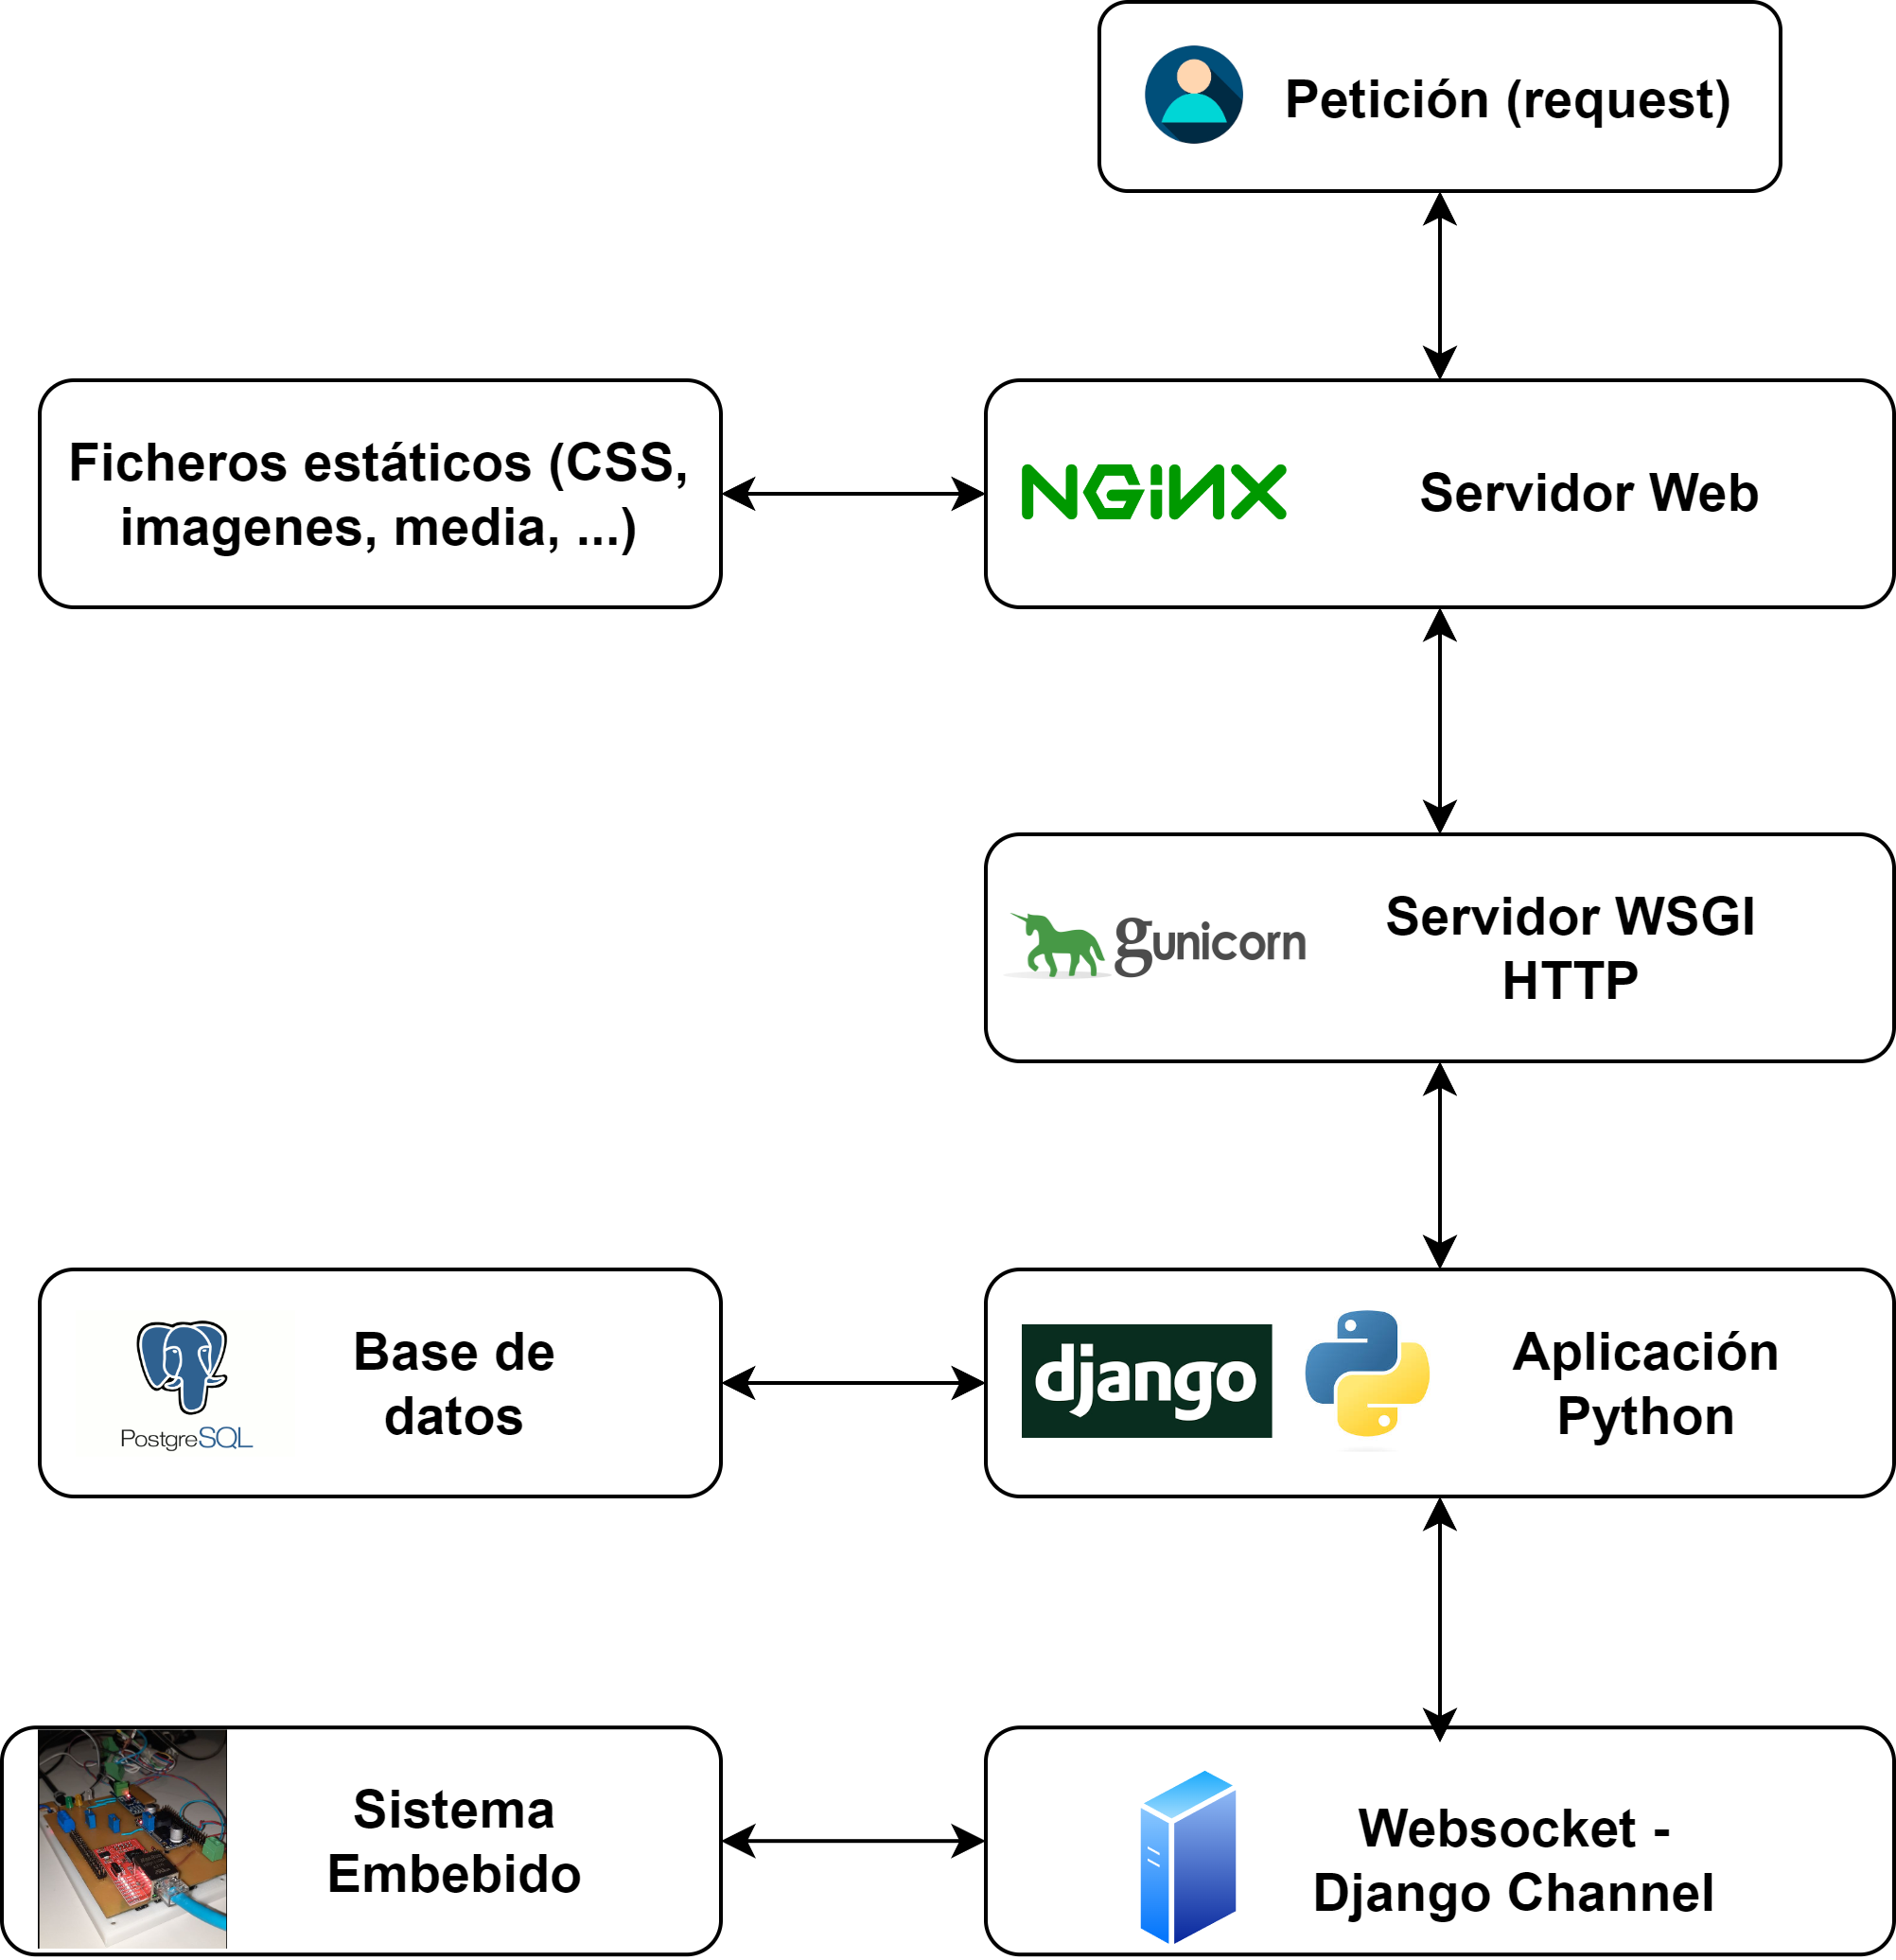
\includegraphics[width=0.7\linewidth]{Figuras/AplicacionWeb/arquitecturaSoft.png}
    \caption{Arquitectura del software implementada.}
    \label{fig:arquitecturaSoft}
\end{figure}

\subsection{Back End}\label{sec:back_end}

Se empleó el patrón de diseño MVT (Modelo-Vista-Plantilla), ilustrado en la Figura \ref{fig:patronMVT}. Este patrón es ampliamente utilizado en el desarrollo web con el marco de trabajo Django. El patrón MVT permite una distinción explícita de las responsabilidades, lo que facilita tanto el desarrollo como el mantenimiento del código.

\begin{itemize}
    \item \textbf{Modelo (M)}: Representa la capa de acceso a la base de datos (ORM). Contiene toda la información sobre los datos, cómo acceder a ellos, validarlos, su comportamiento y las relaciones entre ellos.
    \item \textbf{Vista (V)}:  Corresponde a la capa de lógica de negocios. Se encarga de procesar las solicitudes del navegador y recuperar los datos necesarios del modelo. Luego, renderiza la plantilla (template) para mostrar el HTML resultante.
    \item \textbf{Template (T)}: (Plantilla), representa la capa de presentación, es la parte visual de la aplicación. El template integra los datos dinámicos recuperados del modelo y genera el HTML final que se envía al navegado

\end{itemize}
\begin{figure}[H]
    \centering
    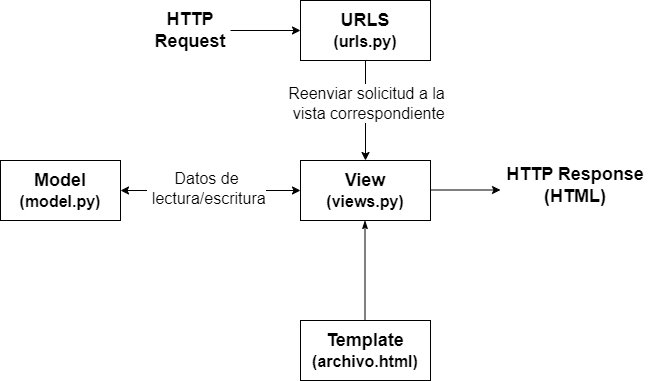
\includegraphics[width=0.8\linewidth]{Figuras/AplicacionWeb/backend/patronMVT.png}
    \caption{Patrón de diseño de software MVT, que divide la lógica del programa en tres elementos interconectados.}
    \label{fig:patronMVT}
\end{figure}


\subsubsection{Base de datos}
Hablar de cuales son las tablas y sus campos y las claves primarias, se puede poner graficos

\begin{figure}[H]
    \centering
    \includegraphics[width=1.1\linewidth]{Figuras/AplicacionWeb/backend/DiagramaEntidadrelacion.png}
    \caption{Diagrama entidad relación}
    \label{fig:DiagramaEntidadRelacion}
\end{figure}



\subsubsection{Generador de trayectoria}
hablar de como el soft calcula la trayectoria en base a los tiempos y puntos ingresados por soft
\subsubsection{Cálculo de incertidumbre}
Acá se puede poner las funciones que se llaman para hacer el calculo de incertidumbre, mostrar un diagrama de flujo desde el inicio con el boton calcular incertidumbre hasta la salida de tablas con los reusltados


\subsection{Frond End}\label{sec:frondEnd}
mas que todo contar como se usa el soft, que aca se entienda como se usa el front
\subsubsection{Carga de metadatos}
que se carga en esta seccion, capturas de pantalla de la vista
\subsubsection{Configuración del sistema}
que se carga en esta seccion, capturas de pantalla de la vista
\subsubsection{Adquisición de datos}
que hace esta seccion como se inicia y para, buscar alguna captura de pantalla

\subsubsection{Procesamiento de datos}
captura de pantalla de los datos crudos, mas su grafico y el boton para calcular la incertidumbre
\subsubsection{Resultados}
mostrar los resultados que muestra el soft como ejemplo usar los del segundo DeltaOHM

\section{Integración con el hardware}
Cuando tenga armado el PCB, hago una prueba de configuración del datalogger, configuración del túnel, metadatos para la calibración

diagrama de como queda todo el sistema, 
\begin{figure}[H]
    \centering
    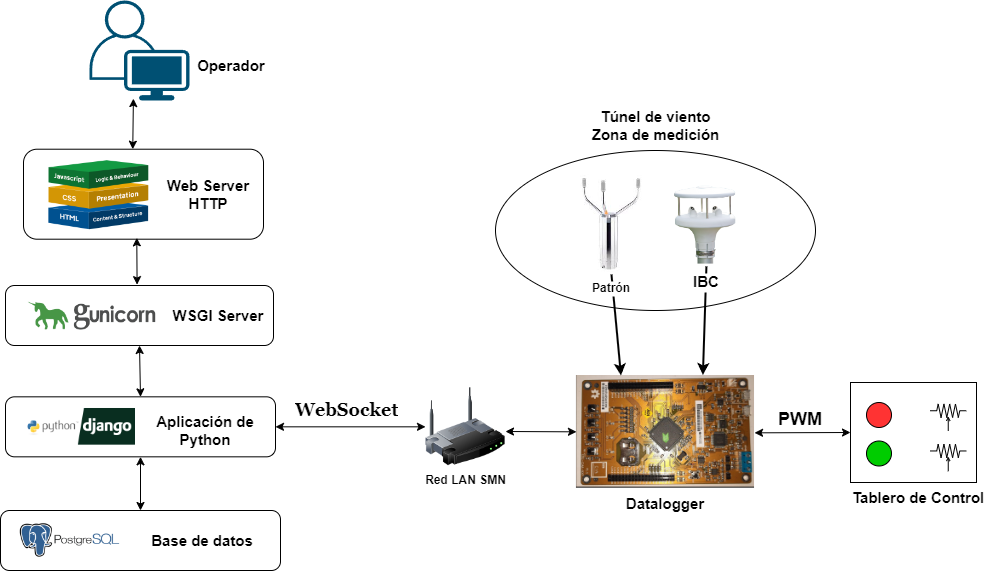
\includegraphics[width=0.9\linewidth]{Figuras/AplicacionWeb/integracionHardware/DiagramaSistemaDesarrollar.png}
    \caption{}
    \label{fig:}
\end{figure}



%-----------------------------------------------------------------------------------------------------
